\section{不变量与算法正确性}
\label{sec:01-Mathematical-Language/04-Induction-and-Recursion/04}

一段训练脚本连跑了三天，损失在降，没有报错。这能说明循环写对了吗？

循环每执行一轮，变量就换一批值，而执行多少轮由输入决定。跑过的是若干条具体轨迹，没跑过的轨迹仍然无穷多。这和上一节开头那份 JSON 文档的处境一样，只是无限的方向从``嵌套多深''换成了``迭代多久''。

先把场景缩到最小，看得清楚些：

\begin{verbatim}
s = 0
k = 0
while k < n:
    k = k + 1
    s = s + k
\end{verbatim}

\(n=5\) 得 15，\(n=10\) 得 55，\(n=100\) 得 5050，都对。但你要的是一句对所有 \(n\) 成立的话。

\subsection{状态也是一步步生成的}

循环有一个和自然数完全同构的生成结构：初始状态 \(s_0\) 是起点，第 \(t\) 轮结束时的状态由第 \(t-1\) 轮的状态经过同一段代码得到。执行到的每个状态，都是初态迭代有限次的产物。

既然生成结构是后继链，论证也就照抄归纳的形状：找一句关于状态的断言，它在起点上为真，并且被``执行一轮''这条规则保住。这句断言就是\textbf{不变量}。

回到那段求和代码。观察轨迹 \((k,s)=(1,1),(2,3),(3,6),(4,10),(5,15)\)，每一项都满足 \(s=k(k+1)/2\)；进入循环之前 \(k=s=0\)，等式同样成立。变量一直在动，它们之间的关系没动。

\begin{center}
\begin{tikzpicture}[x=1cm,y=1cm,>=stealth,font=\small]
  \node[draw,rounded corners,minimum width=2cm] (t) at (0,2.2) {\(k<n\)?};
  \node[draw,rounded corners,minimum width=2cm] (b) at (0,0.6) {循环体};
  \node[draw,rounded corners,minimum width=2cm] (e) at (4.2,2.2) {退出};
  \draw[->] (0,3.5) -- (t);
  \node[right,black!70] at (0.15,3.1) {初始化：\(I\) 成立};
  \draw[->] (t) -- (b);
  \draw[->] (b.west) -- (-2.7,0.6) -- (-2.7,2.2) -- (t.west);
  \node[left,align=right,black!70] at (-2.85,1.4) {保持：\\跑完一轮 \(I\) 仍成立};
  \draw[->] (t.east) -- (e.west);
  \node[above,black!70] at (2.1,2.3) {\(k=n\)};
  \node[below,align=center,black!70] at (4.2,1.85) {终止：\\\(I\) 与 \(k=n\) 一起\\给出结论};
\end{tikzpicture}

\emph{同一句断言要在三个位置成立：进入循环之前、每一轮结束之后、以及退出的那一刻——前两处对应基例与归纳步，第三处负责把它兑换成用户要的结论。}
\end{center}

三个条件放在一起，就是循环正确性的标准检查表：

\begin{itemize}
\tightlist
\item 初始化：第一次判断循环条件之前，不变量成立；
\item 保持：若某轮开始时成立，该轮结束时仍成立；
\item 终止：退出条件与不变量合起来推出想要的结论。
\end{itemize}

前两条只说明``它一直在''，第三条才让它变得有用。

\subsection{把直觉写成推导}

取不变量 \(I\)：\(s=\dfrac{k(k+1)}{2}\) 且 \(0\le k\le n\)。

初始化：\(k=0,s=0\)，等式与范围都成立。

保持：循环体先做 \(k\leftarrow k+1\)，再做 \(s\leftarrow s+k\)，此时 \(k\) 已是新值。设旧值满足 \(I\)，则新的和为 \(\frac{k(k+1)}{2}+(k+1)=\frac{(k+1)(k+2)}{2}\)，正是新 \(k\) 对应的表达式；能进入这一轮说明更新后 \(k\le n\)，范围也保住了。

终止：循环条件是 \(k<n\)，退出时 \(k=n\)，代入得 \(s=n(n+1)/2\)。

和直接对求和公式做数学归纳相比，做的事情是同一件，视角不同。归纳法站在命题一侧，逐个 \(n\) 地推；不变量分析站在程序内部，描述执行到任意中间时刻的变量关系。后者的好处是不必读完整个算法再回头拼归纳假设——不变量就长在执行轨迹上。

\subsection{三个条件各自防住什么}

少了初始化会怎样？把不变量改写成 \(s=\frac{k(k+1)}{2}+7\)，保持步照样一字不差地通过：两边同加 \(k+1\)，常数 7 原样跟过去。可它在进入循环前不成立，于是退出时``推出''的 \(s=n(n+1)/2+7\) 是个假结论。这与上一节里那个加了 7 的求和命题是同一种失效：传递机制完好，只是从没接上真的东西。

保持步失效则更直白，通常来自对更新顺序的误读。上面那段代码若把两行调换成先 \(s\leftarrow s+k\) 再 \(k\leftarrow k+1\)，同一个不变量就保不住了，而它在初始时刻仍然成立——症状要到退出时才暴露。

终止步则约束不变量的强度。写得太弱，比如只保留 \(0\le k\le n\)，前两条轻松通过，退出时却推不出任何关于 \(s\) 的话；写得太强，比如要求每一轮 \(s\) 都等于最终答案，保持步立刻垮掉，因为程序还没跑完。可用的不变量卡在这两条边界之间。

还有一件事这三条管不了：程序会不会停。前三条给出的是\emph{部分正确性}——若程序终止，输出就对。终止性要另外论证，标准做法是上一节末尾提过的那招：找一个取值于自然数、每轮严格下降的量。这里是 \(n-k\)，自然数上不存在无限下降链，所以循环必停。部分正确性加终止性，才是\emph{完全正确性}。

\subsection{不变量从哪儿来}

它不会自己冒出来，得猜，但有几条常用线索。

最常见的一条是``已处理的部分加未处理的部分等于原问题''。二分查找的不变量是``目标若在数组中，必在当前区间内''：左右边界不断收窄，这个包含关系始终没破。Euclid 算法每轮做 \(a\leftarrow b\)、\(b\leftarrow a\bmod b\)，不变量是 \(\gcd(a,b)\) 不变——两个数字在换，它们携带的公约数没换。

另一条是从终止目标往回弱化。若最终要 \(s\) 等于全部 \(n\) 项之和，那么第 \(k\) 轮时 \(s\) 就该等于前 \(k\) 项之和。这正是前面那个不变量的来历。

守恒量也常是好的候选。一批货从仓库 \(A\) 运往 \(B\)，在没有入库、出库和损耗的前提下，\(q_A+q_{\text{在途}}+q_B\) 应当全程守恒。只盯两个仓库的账面库存，货物在运输途中会暂时``消失''，账对不上；把在途状态纳入系统，守恒才成立。反过来，现实若允许破损或盘点修正，就不能硬把``总量恒定''当不变量，得把这些事件写成增减项。好的不变量常常顺带暴露状态模型漏掉了什么。

训练循环里的断言是同一件事的工程写法：概率输出每行和为 1、回放缓冲区长度不超过容量、学习率非负。把它们写进代码，哪一轮第一次触发，就指向破坏了保持步的那段更新。

\subsection{不变量也能说``做不到''}

它更漂亮的用法不是证明程序对，而是证明某件事根本办不成。

从 \(8\times8\) 棋盘上去掉对角两个格子，剩 62 格，能否用 31 块 \(1\times2\) 的骨牌铺满？穷举 31 对格子的排列不现实。改看颜色：棋盘黑白交替，原本各 32 格，而对角两格同色，去掉后成了 30 与 32。

\begin{center}
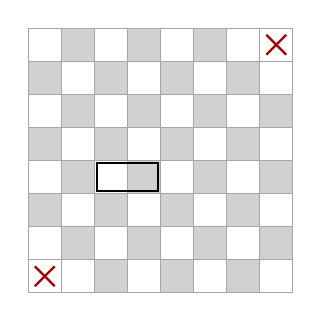
\begin{tikzpicture}[x=0.42cm,y=0.42cm,font=\small]
  \foreach \i in {0,2,4,6}{
    \foreach \j in {0,2,4,6}{
      \fill[black!18] (\i,\j) rectangle ++(1,1);
      \fill[black!18] (\i+1,\j+1) rectangle ++(1,1);
    }
  }
  \fill[white] (0,0) rectangle (1,1);
  \fill[white] (7,7) rectangle (8,8);
  \foreach \i in {0,...,8}{
    \draw[black!35] (\i,0) -- (\i,8);
    \draw[black!35] (0,\i) -- (8,\i);
  }
  \draw[red!65!black,thick] (0.2,0.2) -- (0.8,0.8) (0.2,0.8) -- (0.8,0.2);
  \draw[red!65!black,thick] (7.2,7.2) -- (7.8,7.8) (7.2,7.8) -- (7.8,7.2);
  \draw[thick] (2.08,3.08) rectangle (3.92,3.92);
\end{tikzpicture}

\emph{被划掉的两格同色，而任何摆法的每一块骨牌都必然横跨一深一浅两格。}
\end{center}

每块骨牌无论横放竖放都恰好盖住一深一浅，所以铺过程中``已覆盖的两色格数之差''恒为零。铺满 62 格意味着两色数目相等，与 30 对 32 矛盾。不可能。

一场规模巨大的搜索就这样被压成了两个数字的比较。不用模拟摆放，不用写回溯，一条结构性质就够。

\subsection{它是关系，不是变量}

最后澄清一个常见的混淆。代码里某个变量整个循环期间没被赋值过，它的值当然没变，但这只是一个语法事实，未必能把初始状态和终止结论连起来。真正管用的不变量，牵涉的变量往往一直在跳——\(s\) 和 \(k\) 每轮都变，稳住的是它们之间的关系。不变量长在变量之上，不是在代码里找一个没被写过的名字。

也要承认这套方法的边界。上面给的三条线索都不是算法，找不到合适的不变量并不能说明程序有错，只说明还没找到那句合适的话；而对并发、浮点误差累积或依赖外部状态的循环，光有一句断言往往不够，得先把``状态''本身定义清楚。

回头看这四篇：自然数由后继生成，所以有数学归纳法；树与表达式由构造规则生成，所以有结构归纳；循环状态由迭代生成，所以有不变量。换的是材料，没换的是那句话——论证跟着生成规则走，有限的推理就能覆盖无限的对象。
